\newgeometry{margin=2.5cm}
\section{Conception du projet}
\subsection{Introduction}
\subsection{Diagrammes UML}
\subsubsection{Spécification des acteurs}
L'application SPN-Cars aura trois acteurs :
\paragraph{L'utilisateur régulier}\mbox{} \\
L'utilisateur régulier sera celui qui créera les demandes de transfert, c'est le point focal de l'application.
\paragraph{Le chauffeur}\mbox{} \\
C'est celui qui sera responsable du transfert des clients et livraison de voitures en cas de location de voiture sans chauffeur.
\paragraph{L'admin}\mbox{} \\
L'admin surveillera toutes les opérations en cours, trouvera des solutions s'il y a un problème chez un client et il aura l'autorité de prendre les décisions nécessaires pour assurer les services offerts aux clients.
\subsubsection{Diagramme de cas d'utilisation}
\begin{figure}[H]
    \centering
    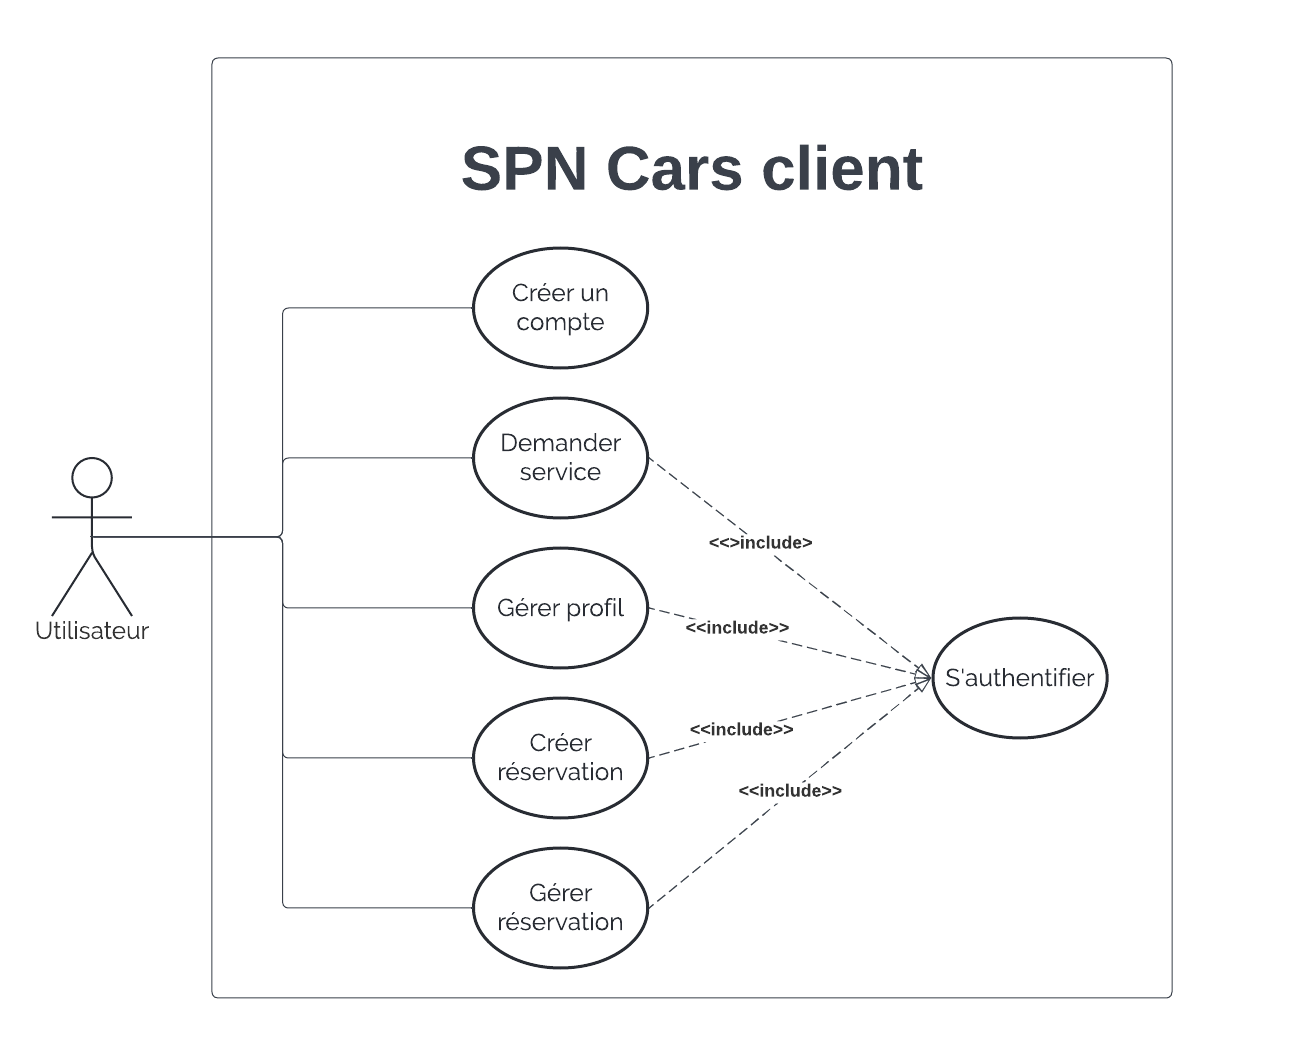
\includegraphics[height=0.8\textheight]{uml/use_cases.png}
    \vspace{1cm}
    \caption{Diagramme de cas d'utilisation}
    \label{fig:use_case_diag}
\end{figure}

\subsubsection{Diagramme de classes}
\begin{figure}[H]
    \centering
    \rotatebox[origin=c]{-90}{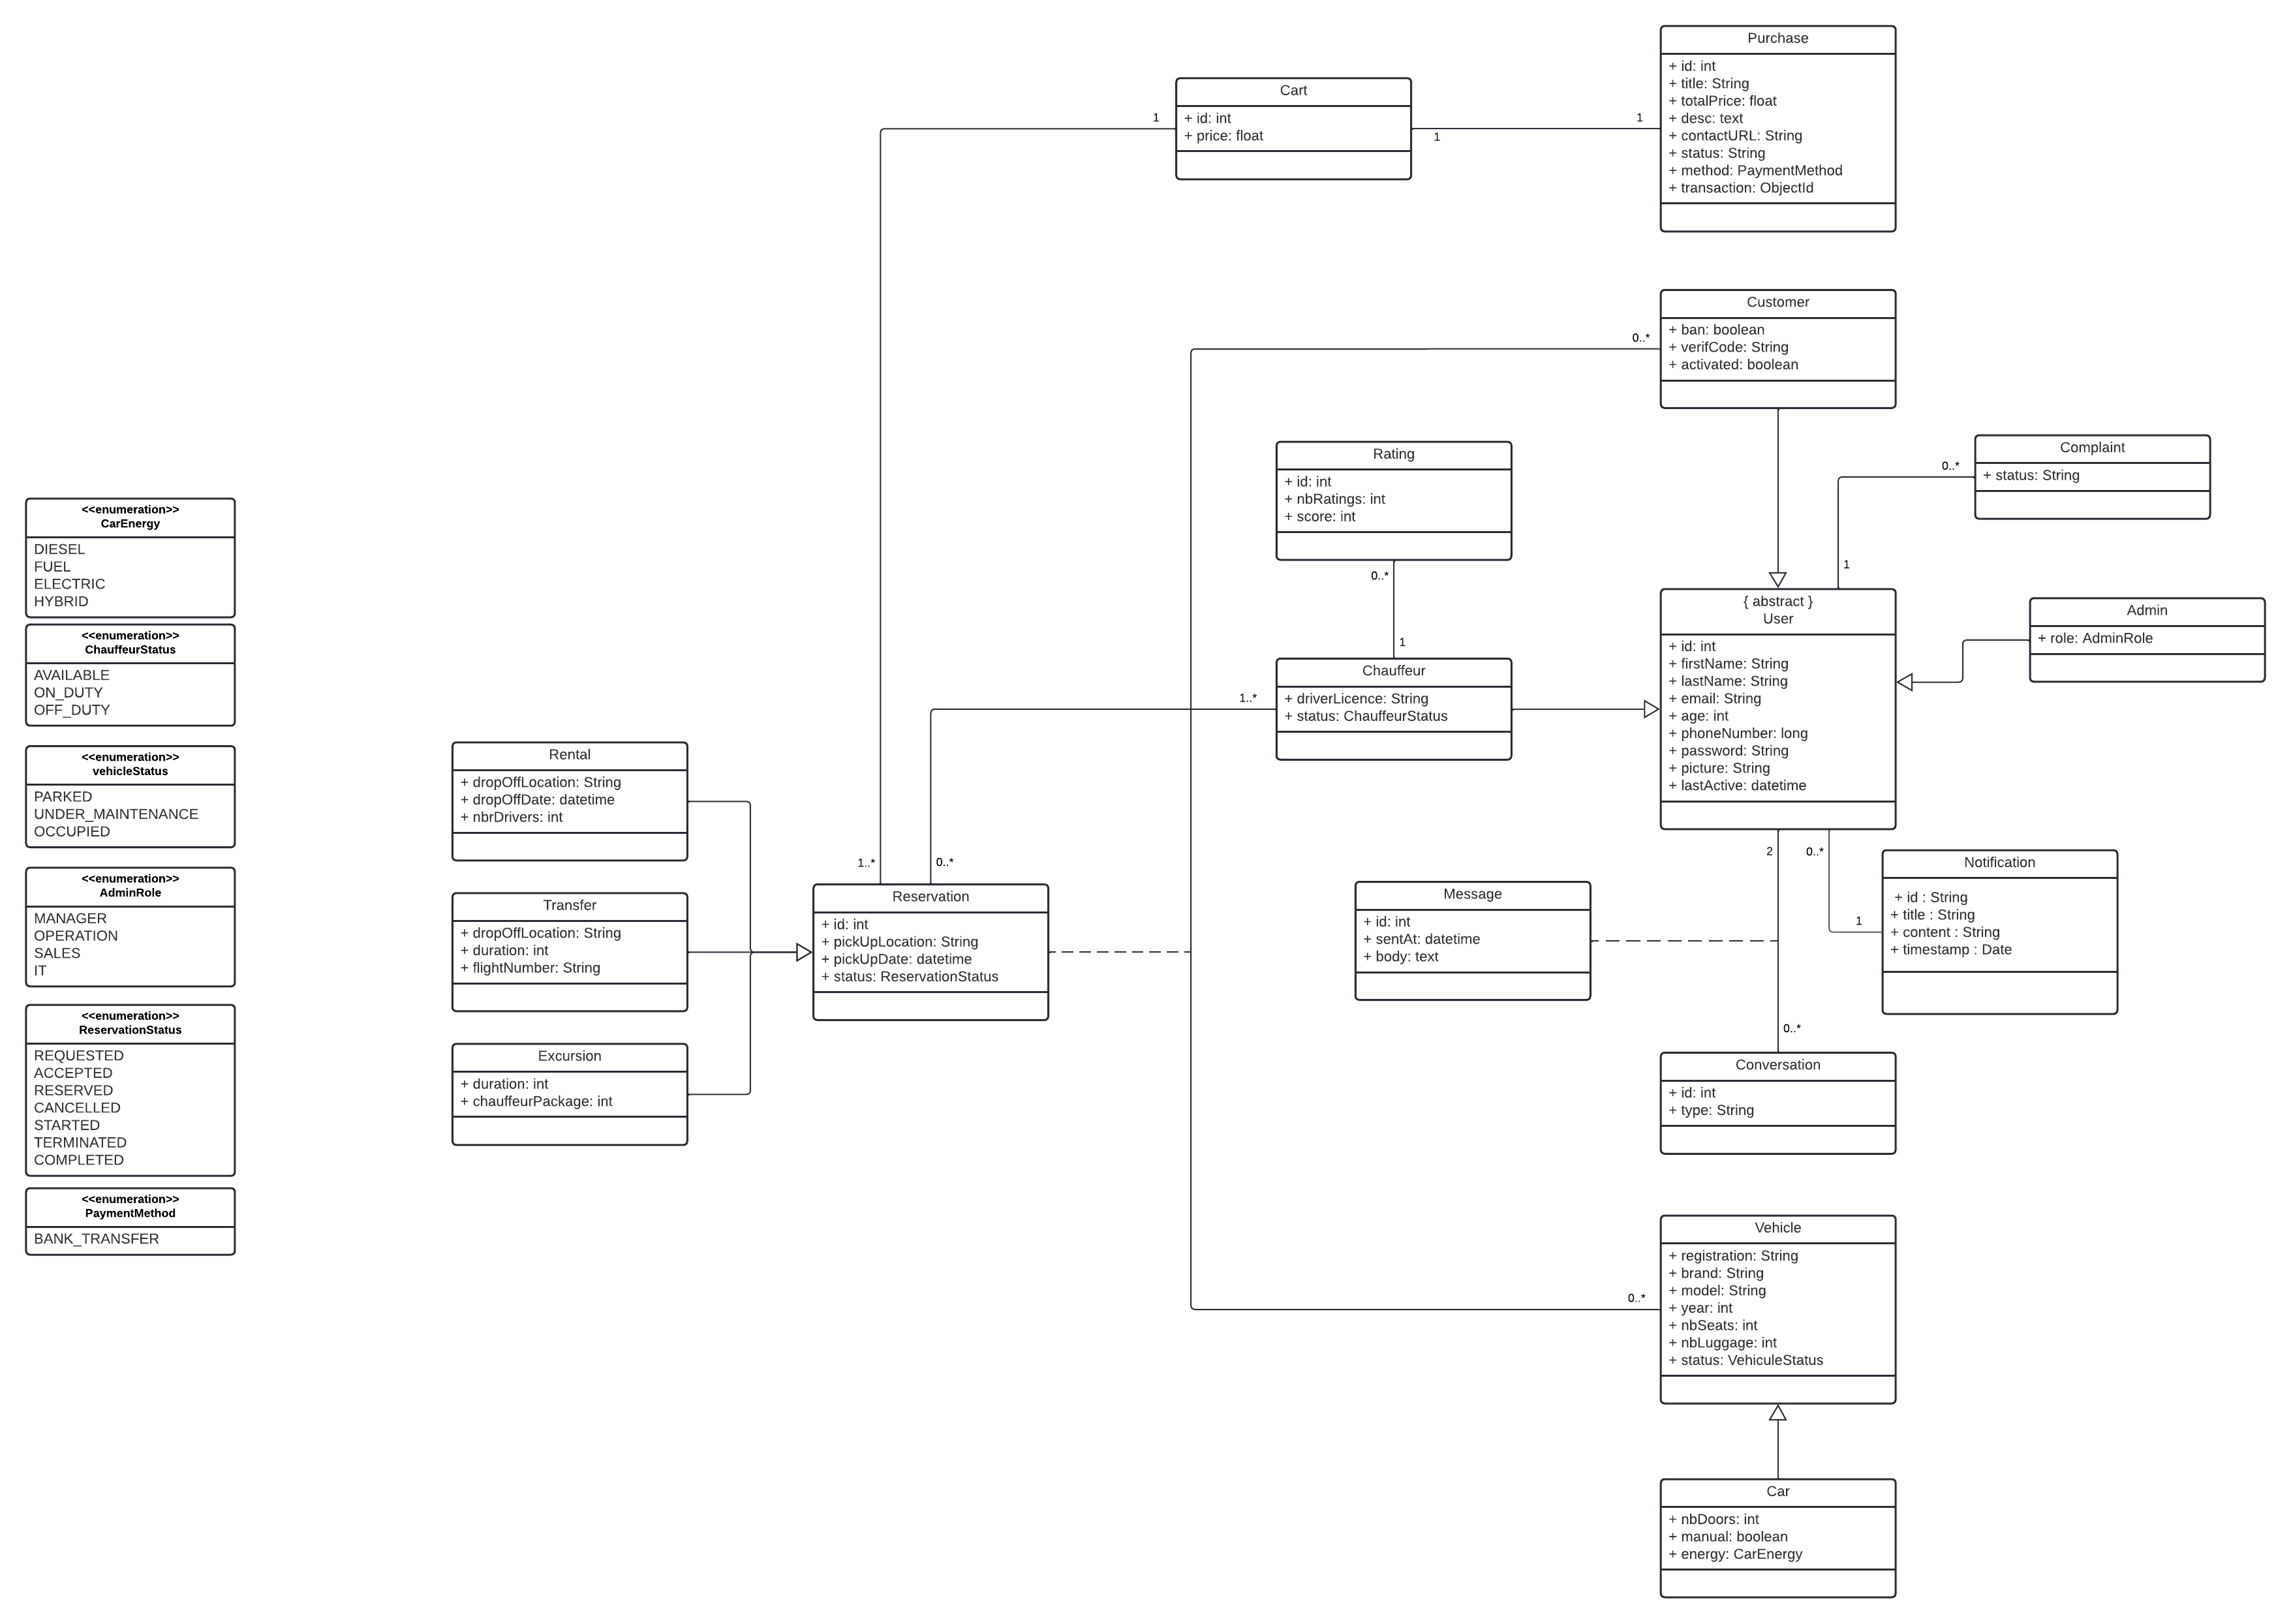
\includegraphics[width=1.2\textwidth]{uml/class_diag.png}}
    \vspace{1cm}
    \caption{Diagramme de classe}
    \label{fig:class_diag}
\end{figure}
\subsection{UI/UX Design}
Avant de passer au développement de l'application, il faut créer d'abord les prototypes des interfaces utilisateur. \\
\noindent Cette étape est nécessaire pour tester plusieurs approches dans les interfaces de l'application, s'assurer d'offrir une expérience utilisateur agréable. \\
\vspace{1cm}
\begin{multicols}{2}
    \begin{figure}[H]
        \centering
        
\includegraphics[width=0.25\textwidth]{ui_screenshots/Guide.png}
        \vspace{1cm}
        \caption{Première page.}
        \label{fig:start_page}
    \end{figure}
    \begin{figure}[H]
        \centering
        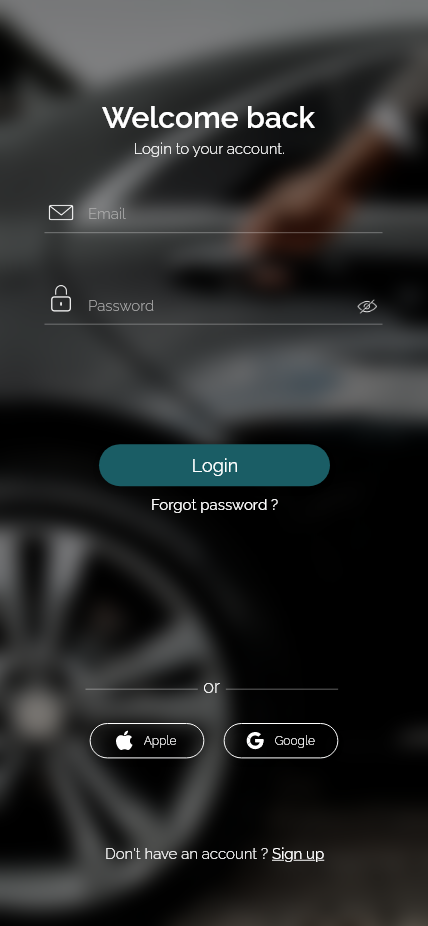
\includegraphics[width=0.25\textwidth]{ui_screenshots/sign in.png}
        \vspace{1cm}
        \caption{Page de connexion.}
        \label{fig:sign_in_page}
    \end{figure}
\end{multicols}
\newpage
\begin{multicols}{2}
    \begin{figure}[H]
        \centering
        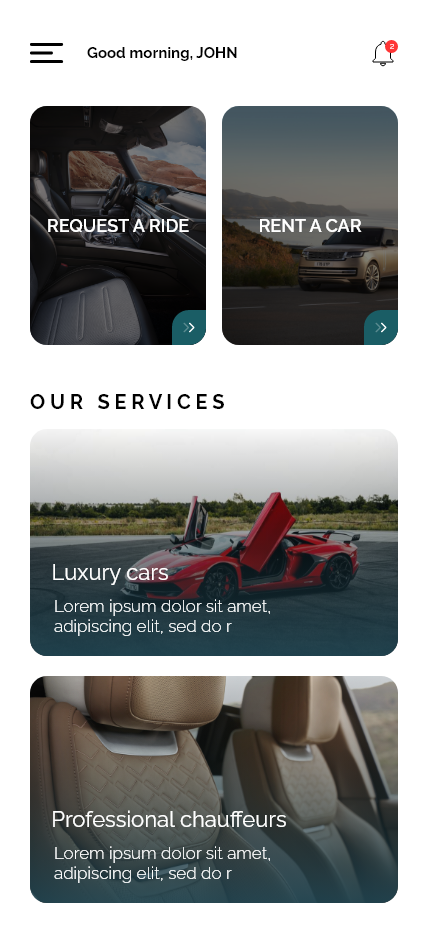
\includegraphics[width=0.25\textwidth]{ui_screenshots/No Active trip.png}
        \vspace{1cm}
        \caption{\centering Page d'accueil.}
        \label{fig:no_active_trip}
    \end{figure}
    \begin{figure}[H]
        \centering
        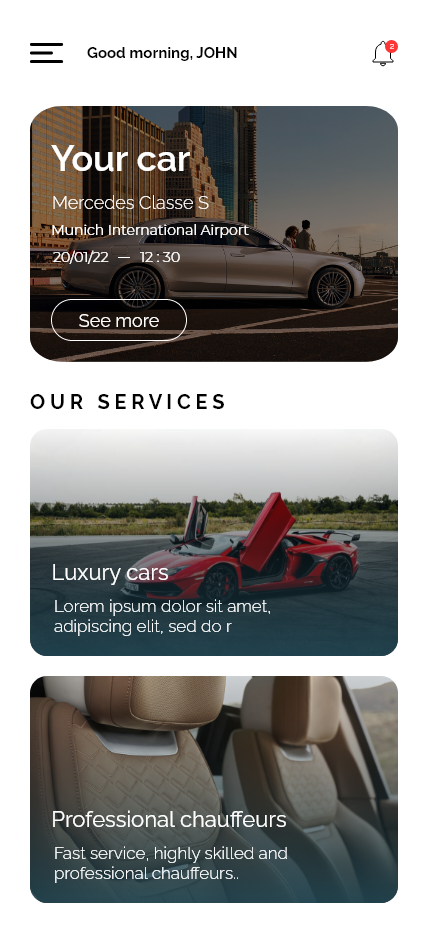
\includegraphics[width=0.25\textwidth]{ui_screenshots/Active trip.png}
        \vspace{1cm}
        \caption{\centering Page d'accueil lors d'un transfert en cours.}
        \label{fig:active_trip}
    \end{figure}
\end{multicols}
\begin{multicols}{2}
    \begin{figure}[H]
        \centering
        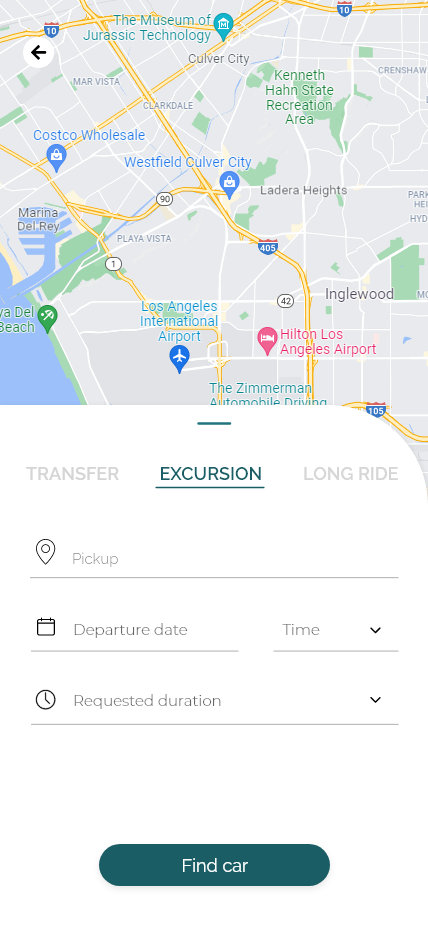
\includegraphics[width=0.25\textwidth]{ui_screenshots/Excursion.png}
        \vspace{1cm}
        \caption{\centering Sélection de type de transfert.}
        \label{fig:trip_select}
    \end{figure}
    \begin{figure}[H]
        \centering
        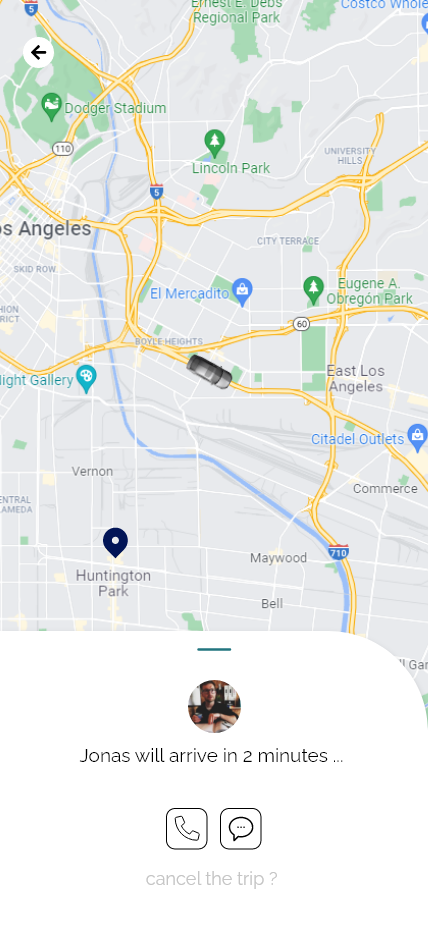
\includegraphics[width=0.25\textwidth]{ui_screenshots/Map view.png}
        \vspace{1cm}
        \caption{\centering Suivi de la position actuelle du chauffeur avec la voiture.}
        \label{fig:follow_driver}
    \end{figure}
\end{multicols}
\newpage
\begin{multicols}{2}
    \begin{figure}[H]
        \centering
        \includegraphics[width=0.25\textwidth]{ui_screenshots/Available cars – 1.png}
        \vspace{1cm}
        \caption{\centering Liste de voitures disponibles.}
        \label{fig:available_cars}
    \end{figure}
    \begin{figure}[H]
        \centering
        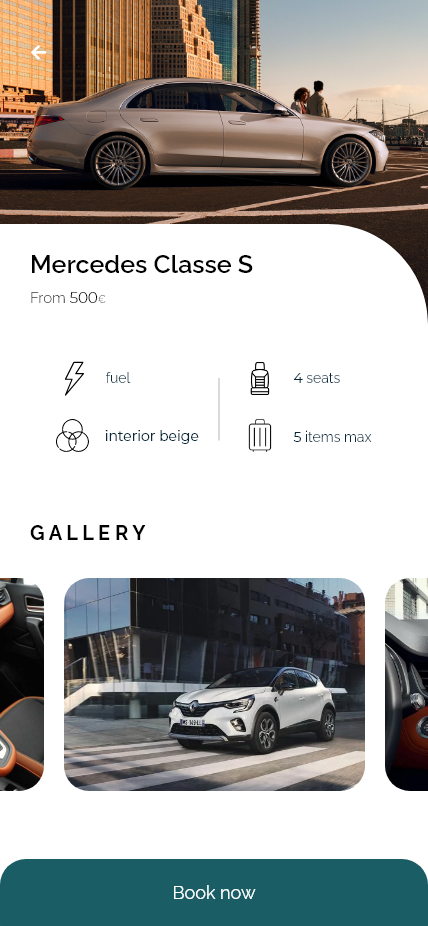
\includegraphics[width=0.25\textwidth]{ui_screenshots/Car details.png}
        \vspace{1cm}
        \caption{\centering Détails de la voiture sélectionnée.}
        \label{fig:car_details}
    \end{figure}
\end{multicols}
\vspace{1cm}
\begin{figure}[H]
    \centering
    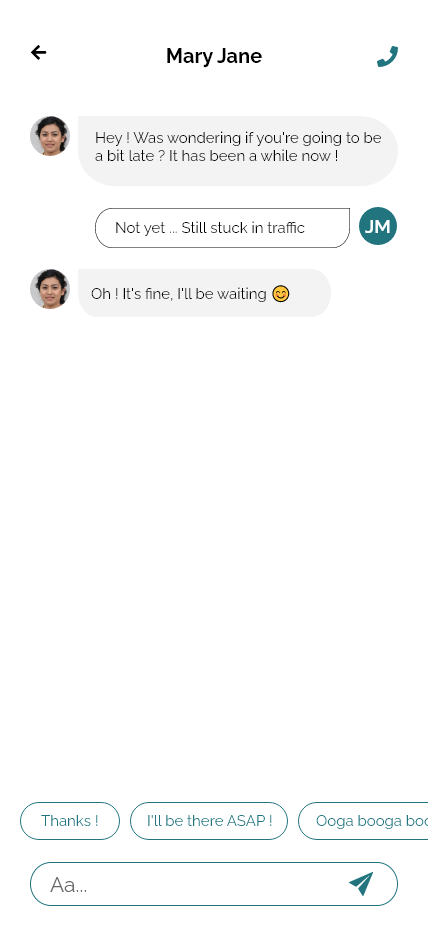
\includegraphics[width=0.25\textwidth]{ui_screenshots/DMs.png}
    \vspace{1cm}
    \caption{\centering Messagerie instantannée avec le chauffeur.}
    \label{fig:dms}
\end{figure}

\subsection{Technologies et logiciels utilisés}
Comme cette application sera une application mobile, il est nécessaire que la performance soit la priorité lors du développement. C'est pourquoi on a choisi les technologies suivantes pour offrir une application rapide, performante, facile à utiliser.\\
\noindent Ses différentes technologies sont classifiés dans trois domaines principalement : Conception des interfaces graphiques, développement de l'application, et développement du back-end de l'application.\\
\subsubsection{Adobe Xd}
\vspace{1cm}
\begin{figure}[H]
    \centering
    
\includegraphics[width=0.25\textwidth]{xd_logo.png}
    \vspace{1cm}
    \caption{Logo Adobe Xd}
    \label{fig:xd_logo}
\end{figure}
\textit{\textbf{Adobe Xd}} est un outil de conception et modélisation des interfaces utilisateur des applications web et mobiles, développé par Adobe Inc.\\
\noindent Grâce aux outils fournis par Adobe Xd, la conception, l'amélioration et la rectification des interfaces graphiques et l'expérience de l'utilisateur de l'application sera plus facile, plus rapide et plus efficace.
\noindent Dans le cadre de ce projet, Adobe Xd a été utilisé pour la création des prototypes des interfaces graphiques, qui seront, par la suite, construits en application mobile à l'aide de Flutter.
\subsubsection{Flutter}
\vspace{1cm}
\begin{figure}[H]
    \centering
    
\includegraphics[width=0.25\textwidth]{flutter.png}
    \vspace{1cm}
    \caption{Logo Flutter}
    \label{fig:flutter_logo}
\end{figure}
\textit{\textbf{Flutter}} est un kit de développement (SDK) open-source créé par Google et publié en 2017.\\
\noindent Flutter permet de créer des application mobiles (Android / iOS), web et meême desktop (Windows / Linux / MacOS), avec une seule base de code en Dart, un langage de programmation développé aussi par Google. \\
\noindent Flutter présente plusieurs avantages qui permettent de créer des applications mobiles performantes et réduit aussi le coût et le temps de développement nécessaires, grâce au langage de programmation utilisé \textit{\textbf{Dart}} qui est très facile à maîtriser et qui offre plusieurs avantages, dont le plus important la fonctionnalité de <<\textit{\textbf{Hot Reload}}>> qui permet de recharger l'application et afficher les changements sur l'écran sans passer par la recompilation du code source.
\subsubsection{Express JS}
\vspace{1cm}
\begin{figure}[H]
    \centering
    
\includegraphics[width=0.25\textwidth]{express.png}
    \vspace{1cm}
    \caption{Logo Express}
    \label{fig:express_logo}
\end{figure}
\textit{\textbf{Express JS}} est un framework back-end gratuit et open-source pour NodeJS. Créé par TJ Holowaychuk, la première version publique d'Express JS a été introduite au public en 2010.\\
Express JS est un framework minimaliste, très léger pour garantir une performance optimale et une exécution rapide. Ce framework est aussi très flexible, même s'il fournit que quelques fonctionnalités, grâce à \textit{\textbf{NPM}}, le gestionnaire de packets de NodeJS, il peut être complété par plusieurs librairies disponibles.\\
\noindent Grâce à son minimalisme et facilité d'implémentation, ExpressJS est utilisé par plusieurs par nombreuses sociétés dans le monde, pour développer tout type d'applications, parmi ses sociétés il y a des géants de technologies tels que \textit{\textbf{IBM}}, \textit{\textbf{Uber}}, et plusieurs autres.
\subsubsection{MongoDB}
\vspace{1cm}
\begin{figure}[H]
    \centering
    
\includegraphics[width=0.25\textwidth]{mongo.png}
    \vspace{1cm}
    \caption{Logo MongoDB}
    \label{fig:mongo_logo}
\end{figure}
\textit{\textbf{MongoDB}}, est un système de gestion de base de données NoSQL, orientée documents. Une base de données NoSQL est utilisée pour le stockage de volumes massifs de données, elle se distingue des des bases de données relationnelles par sa flexibilité et ses performances.\\
\noindent Le système MongoDB est développé par la société qui porte le même nom en 2007. Cette entreprise travaillait sur un système de cloud computing à données largement réparties.\\
\noindent Il est depuis devenu l'un des systèmes de gestion de base de données les plus utilisées, notamment pour des sites web très populaires tels que : \textit{\textbf{SourseForge.net}}, \textit{\textbf{eBay}} et \textit{\textbf{The New York Times}}.\\
\noindent Contrairement à une base de données relationnelle SQL traditionnelle, MongoDB ne repose pas sur des tableaux et des colonnes. Les données sont stockées sous forme de collections et de documents.
Les documents sont des paires de valeurs / clés servant d'unité de données de base. Les collections quant à elles contiennent des ensembles de documents et de fonctions. Elles sont l'équivalent des tableaux dans les bases de données relationnelles classiques.
\subsubsection{Firebase}
\vspace{1cm}
\begin{figure}[H]
    \centering
    
\includegraphics[width=0.25\textwidth]{firebase.png}
    \vspace{1cm}
    \caption{Logo Firebase}
    \label{fig:firebase_logo}
\end{figure}
\textit{\textbf{Firebase}} est une plateforme créée en 2011, puis acquise et développée par Google en 2014. Firebase facilite la création de back-end à la fois scalable et performant.\\
\noindent L'objectif de firebase est d'offrir aux professionnels et aux particuliers un moyen d'éviter l'engagement dans un processus complexe de création et de maintenance d'une architecture serveur.\\
\noindent Firebase offre des API intuitives regroupées dans un SDK unique. Ces API permettent de gagner du temps et de réduire le nombre d'intégrations qu'on doit gérer dans l'application.\\
\noindent Firebase offre plusieurs services que tout le monde peut utiliser gratuitement grâce à sa politique <<pay as you go>> qui nécessite le paiement de ses services seulement si l'utilisation des ressources dépasse le quota du plan gratuit offert. Les services de Firebase les plus utilisés sont :
\begin{itemize}
    \item \textbf{Realtime Database}: Une base de données NoSQL, bénéficiant d'un hébergement cloud et permettant le stockage et la synchronisation de données des untilisateurs.
    \item \textbf{Fireabse Authentification}: Un SDK prêt et facile à exploiter qui permet de d'authentifier les utilisateurs en offrant plusieurs méthodes d'authentification tels que Google, Apple, Facebook, Email et mot de passe, numéro de téléphone et plusieurs d'autres méthodes pour assurer l'authentification de l'utilisateur.
    \item \textbf{Firebase Cloud Messaging}: Permet de connecter plusieurs périphériques au serveur dans les meilleures conditions (fiabilité et économie de batterie). Ce service permet de recevoir et envoyer des notification sur les différentes plateformes (Web / iOS / Android). Avec Firebase Cloud Messaging, il est possible aussi d'assurer un service de messagerie instantanée entre les utilisateurs.
\end{itemize}
\subsubsection{Git}
\vspace{1cm}
\begin{figure}[H]
    \centering
    
\includegraphics[width=0.25\textwidth]{git.png}
    \vspace{1cm}
    \caption{Logo Git}
    \label{fig:git_logo}
\end{figure}
\textit{\textbf{Git}} est un système de contrôle de version open-source créé en 2005 par \textit{\textbf{Linus Torvalds}}, le créateur du noyau du système d'exploitation Linux.\\
\noindent Un logiciel de versioning, ou logiciel de gestion de version est un logiciel qui permet de conserver un historique des modifications effectuées sur un projet afin de pouvoir rapidement identifier les changements effectuées et de revenir à une ancienne version en cas de problème.\\
\noindent Git permet de gérer les ajouts et changements apportés au code source de manière tracée. Ainsi, si une erreur est commise, les développeurs peuvent revenir en arrière et comparer les versions antérieures du code, ce qui leur permet de corriger l'erreur tout en minimisant les perturbations pour tous les membres de l'équipe.



